\chapter{Architectural Design}

\section{Overview}
The CKB platform system is composed by a 3-tier architecture.\\
Its software application architecture is organized into three logical tiers: the presentation tier, or user interface; the application tier, where data is processed; and the data tier, where the data associated with the application is stored and managed.

\begin{figure}[H]
    \centering
    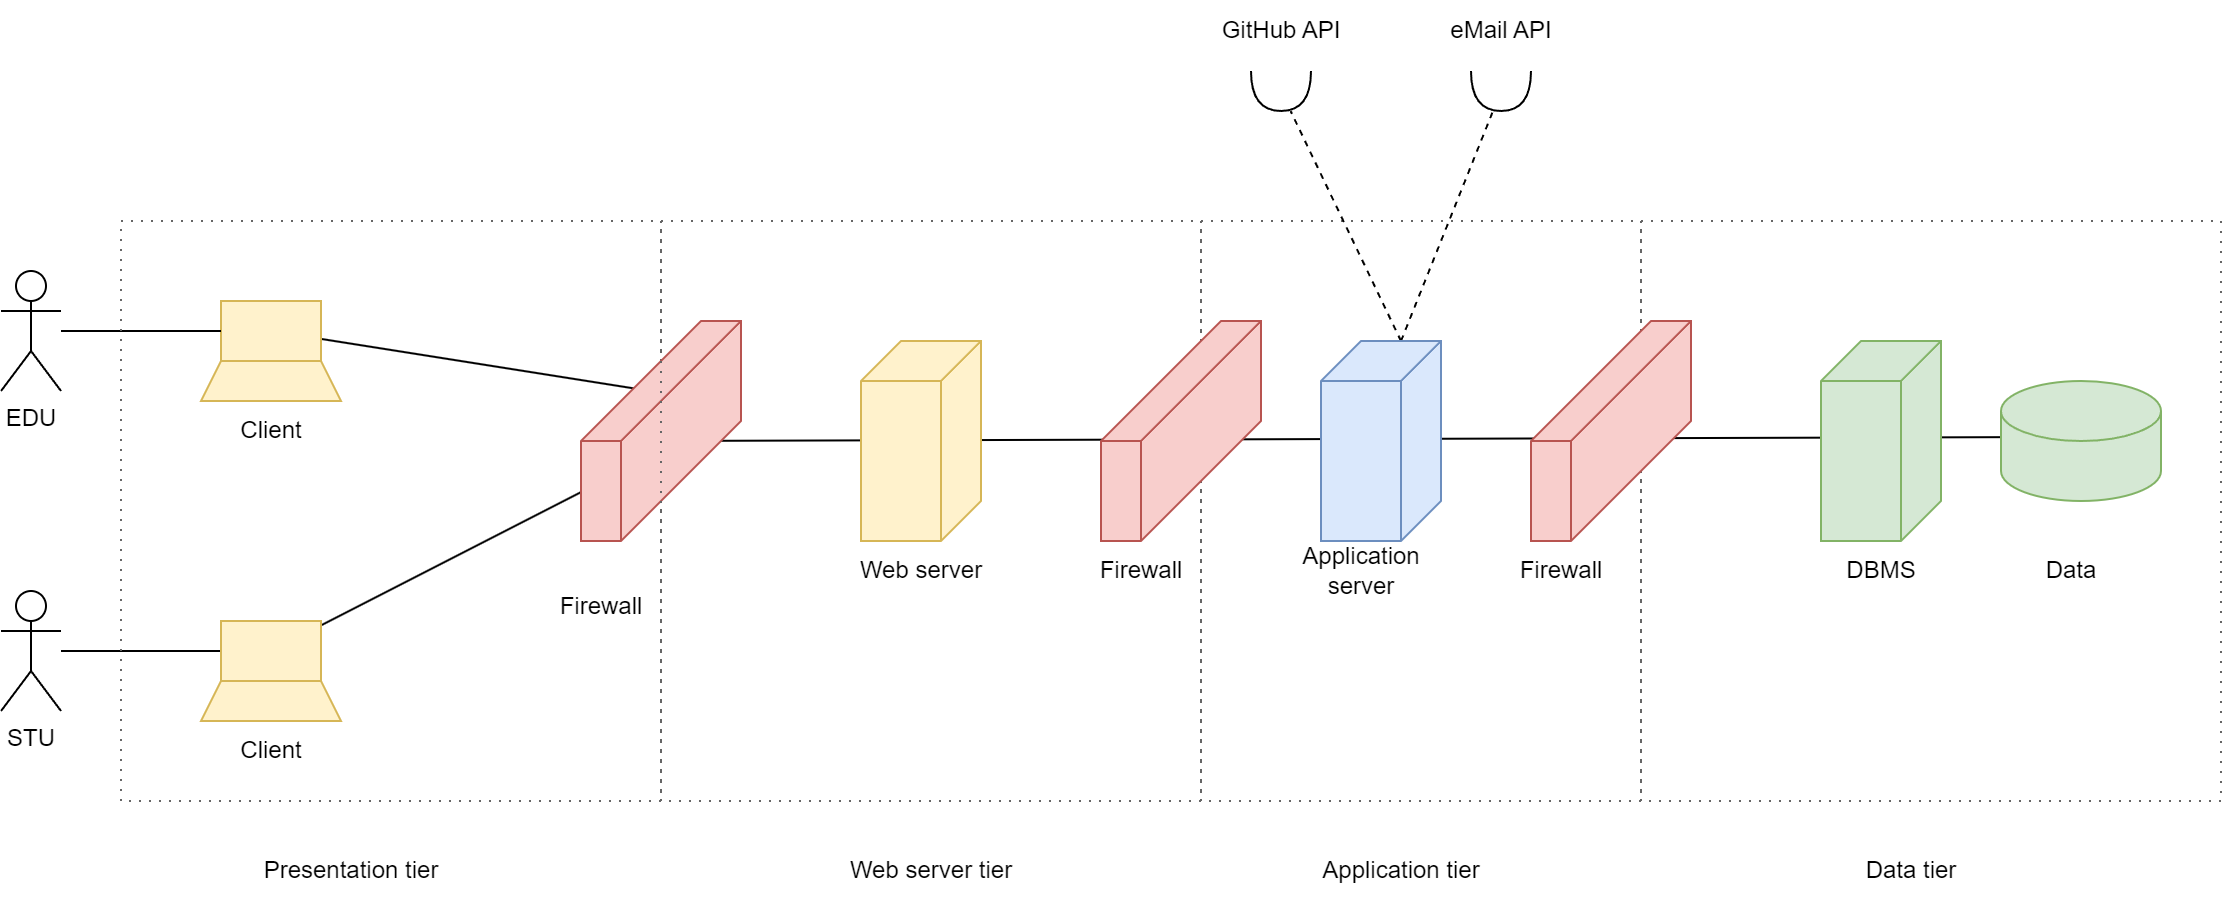
\includegraphics[width=\textwidth]{images/diagrams/high_level_diagram.png}
    \caption{High level components diagram}
\end{figure}

The service will be accessed through a web interface, employing a Single Page Application (SPA). Utilizing an SPA is ideal for this application, as it facilitates extensive interaction without necessitating frequent page reloads.\\
The system's architecture is structured into distinct layers, with application servers interacting with a database management system and utilizing APIs for data retrieval and storage. Adhering to REST standards, the application servers are intentionally designed to be stateless, handling the login sessions for user thanks to the caching, following the best practices for web applications.\\
The system will include more than one firewall to ensure security.\\

\section{Component view}
The system is composed by the following components:

\begin{figure}[H]
    \centering
    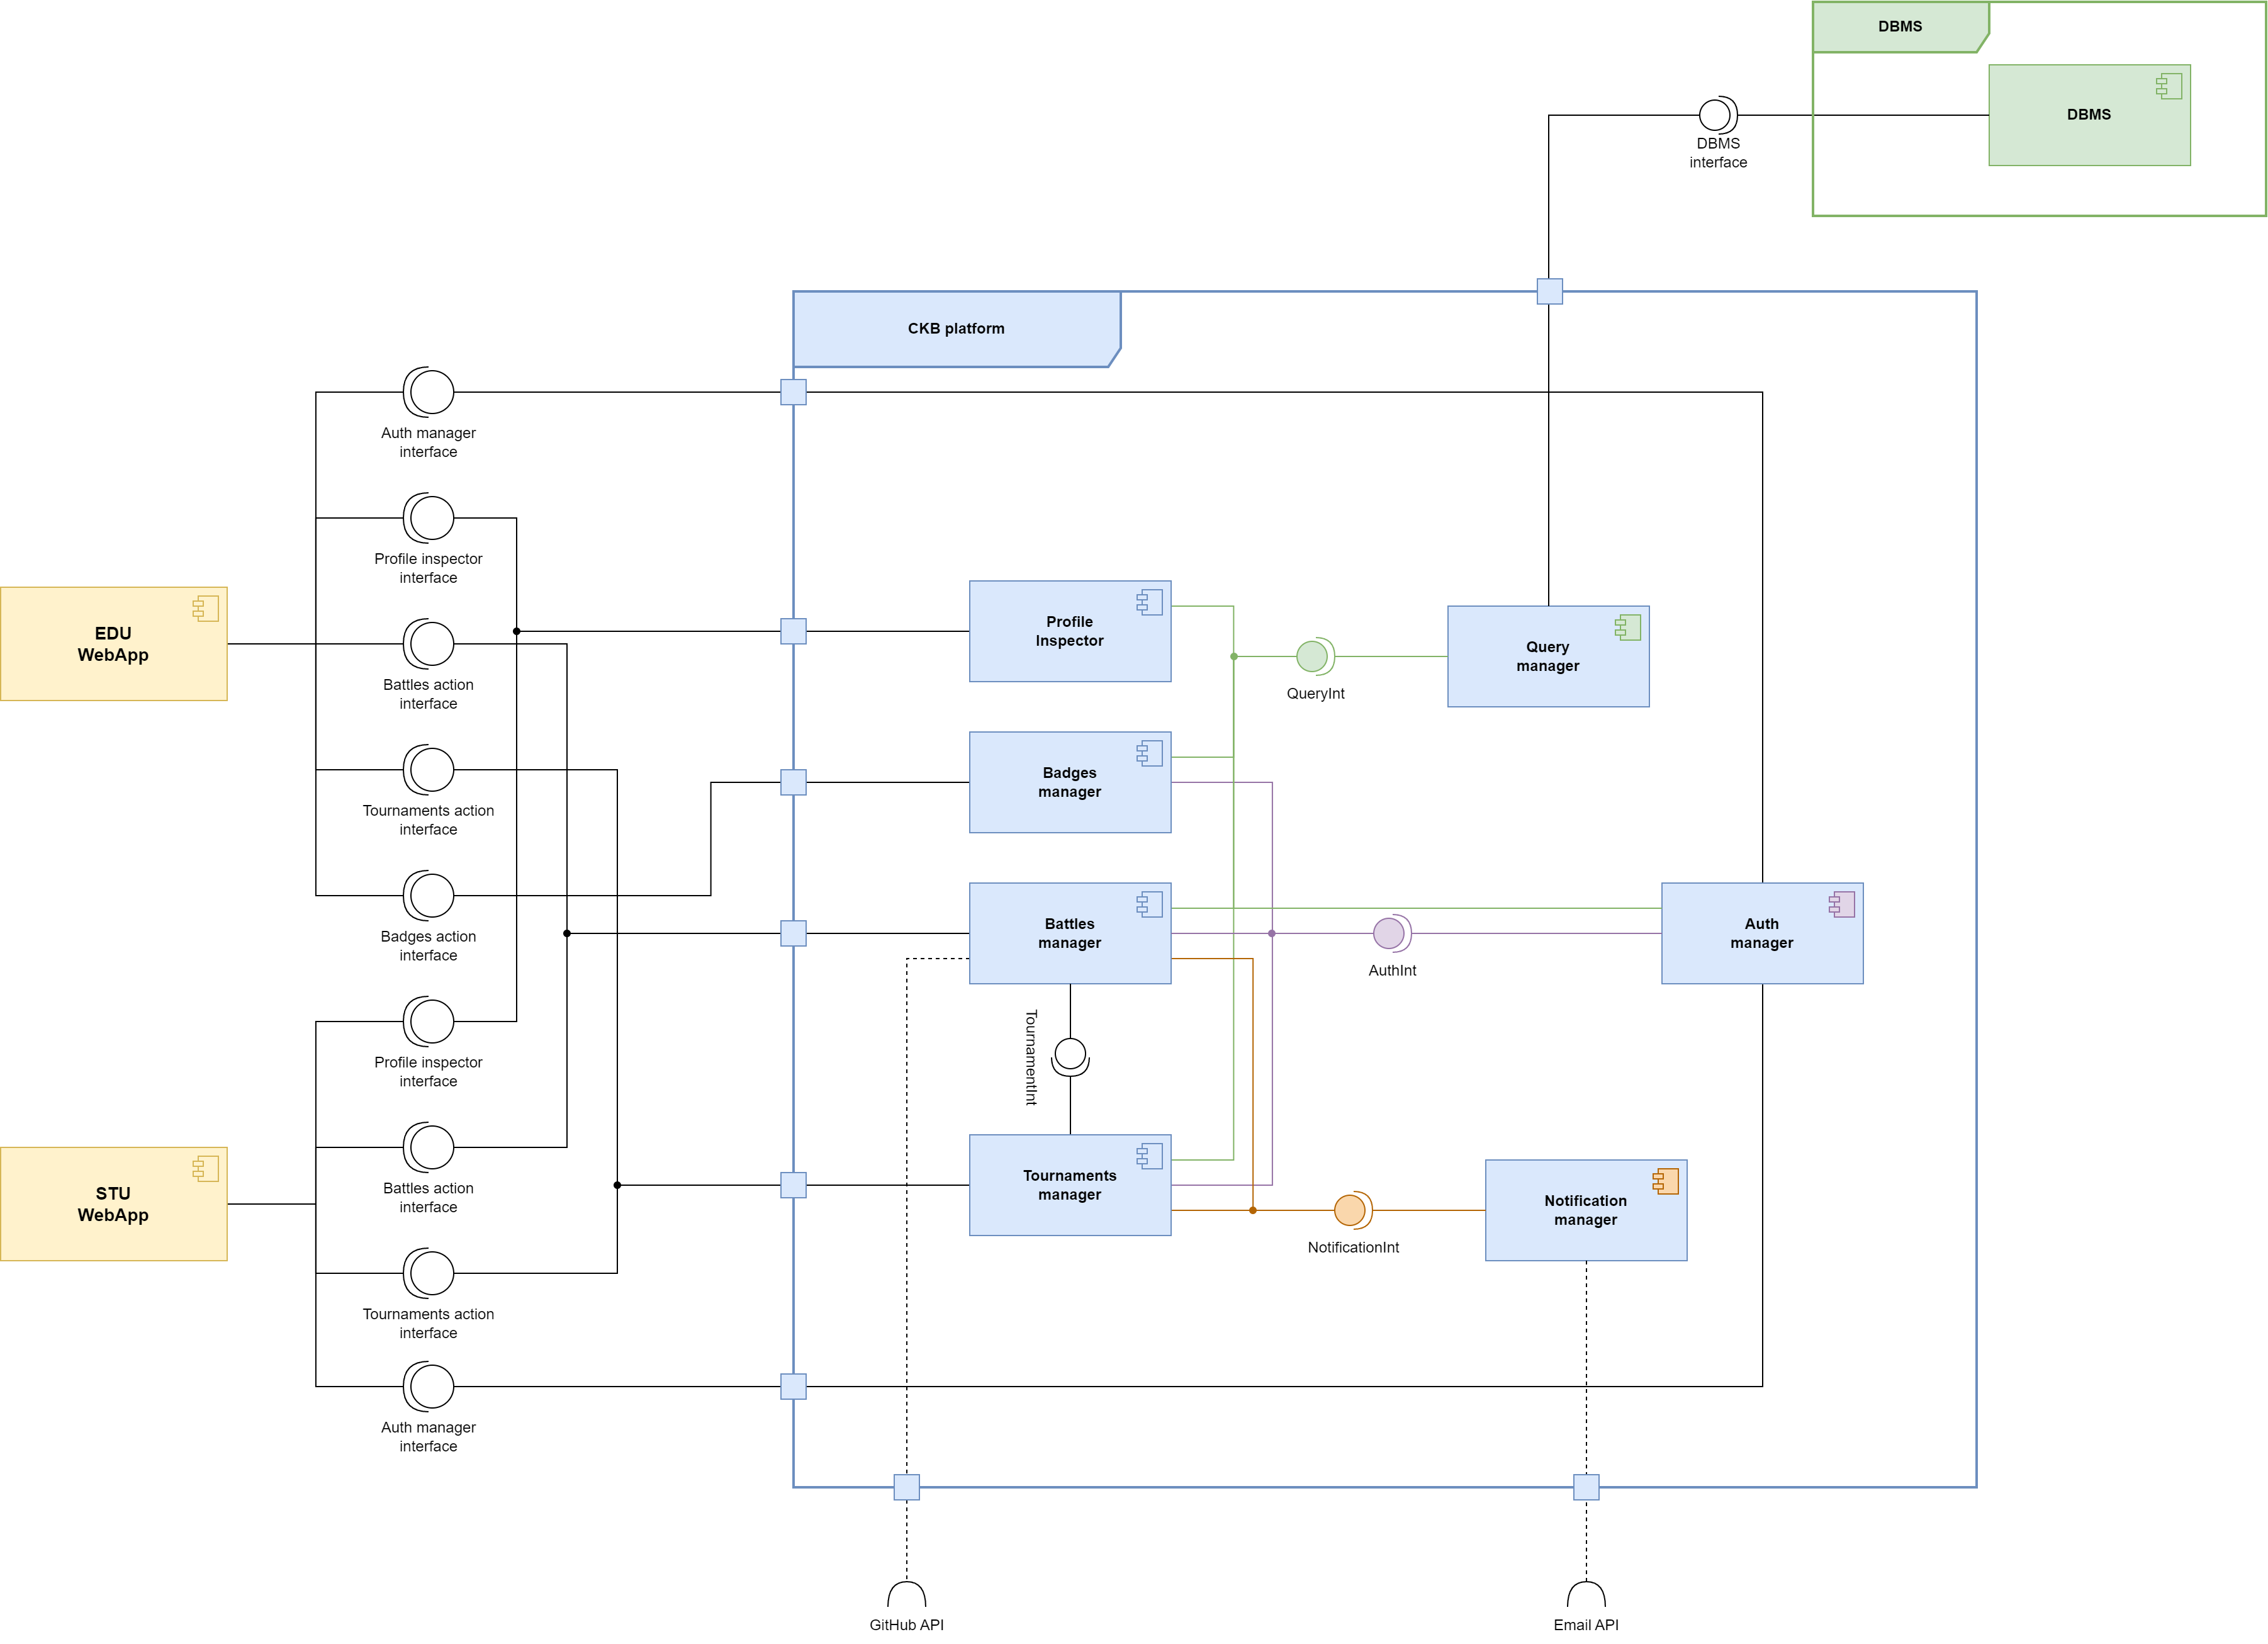
\includegraphics[width=\textwidth]{images/diagrams/component_diagram.png}
    \caption{Component diagram}
\end{figure}

In order to maintain the readability of the diagram, the interfaces have been grouped with respect to their functionality; the complete set of endpoints is available later in the document.\\

\subsection{Client components}

The client components are represented by only a single component, a user-friendly WebApp, that will behave differently depending on the type of the user that is using it (whether it is an EDU or a STU).\\
The WebApp is interfaced with the server components through all the APIs offeded by the server (see later for a detailed description of the APIs).\\

\subsection{Server components}

\subsubsection*{Query manager}
The query manager is the component that handles the queries made by the other components that need to access the database. It is responsible for the execution of the queries and for the communication with the database.\\
It is interfaced with all the internal models of the system that need to access the database, i.e. all the other components of the system exept for the notification manager.\\
It is interfaced with the database through the DBMS API, external to the system.

\subsubsection*{Auth manager}
The auth manager is the component that handles the authentication of the users and the authorization of the requests made by the other components that need to access the database with respect to the user that made the request.\\
It is interfaced with all the internal models of the system that behave differently depending on the level of the user that made the request, i.e. the badges manager, the tournament manager and the battle manager.\\
It isn't interfaced with any external component.

\subsubsection*{Notification manager}
The notification manager is the component that handles the need of the system to notify the users of some events, such as the start of a tournament or the end of a battle.\\
It is interfaced with all the internal models of the system that need to notify the users, i.e. the tournament manager and the battle manager.\\
It is interfaced with the Email API, external to the system.

\subsubsection*{Badges manager}
The badges manager is the component that handles the gamification badges.\\
It allows:
\begin{itemize}
    \item the creation of new badges;
    \item the assignment of badges to the STUs;
\end{itemize}
{\color{red}Qui devo interfacciare anche con battle e user?}
It is interfaced with the auth manager (since the creation of a badge is admissible only for the EDUs) and with the query manager (since it needs to access the database to store the badges).\\
It is interfaced with the EDU WebApp through the proprer, external to the system.

\subsubsection*{Tournaments manager}
The tournament manager is the component that handles the management of the tournaments.\\
It allows:
\begin{itemize}
    \item the creation of new tournaments;
    \item the closure of the torunaments
    \item the visualization of the tournaments;
    \item the excange of admin permission between EDUs;
    \item the subscription of the STUs to the tournaments;
    \item the visualization of the scores of the STUs in the tournaments, and so of the ranking
    \item the visualization of the battles within a tournament
\end{itemize}
It is interfaced with the auth manager (to allow and perform different actions depending on the level of the user that made the request), with the query manager (since it needs to access the database) and the notification manager (since it needs to notify the users of the start and the end of a tournament).\\
It is interfaced with the WebApp, both EDU and STU, through the proper APIs, external to the system.

\subsubsection*{Battles manager}
{\color{red} specificare meglio}
The battles manager is the component that handles the management of the battles.\\
It allows:
\begin{itemize}
    \item the creation of new battles;
    \item the subscription of the STUs to the battles;
    \item the visualization of the scores of the teams in the battles, and so of the ranking
    \item the visualization of the battles;
    \item the automatic evaluation of the battles;
    \item the eventual manual evaluation of the battles by the EDUs
\end{itemize}
It is interfaced with the auth manager (to allow and perform different actions depending on the level of the user that made the request), with the query manager (since it needs to access the database) and the notification manager (since it needs to notify the users of the opening of subscriptions, the start and the end of a bettle).\\
It is interfaced with the WebApp, both EDU and STU, through the proper APIs and with GitHub (to perform the manual evaluation), all external to the system.

\subsubsection*{Profile Inspector}
The profile inspector is the component that handles the visualization of the profiles of the STUs and, consequently, of the badges that a STU has earned during the battles and the tournaments.\\
It is interfaced with the query manager (since it needs to access the database).
It is interfaced with the WebApp, both EDU and STU, through the proper APIs, external to the system.

\subsection{Logical description of the data}
The data of the system is organized in a relational database, with the following entity-relationship diagram:

\begin{figure}[H]
    \centering
    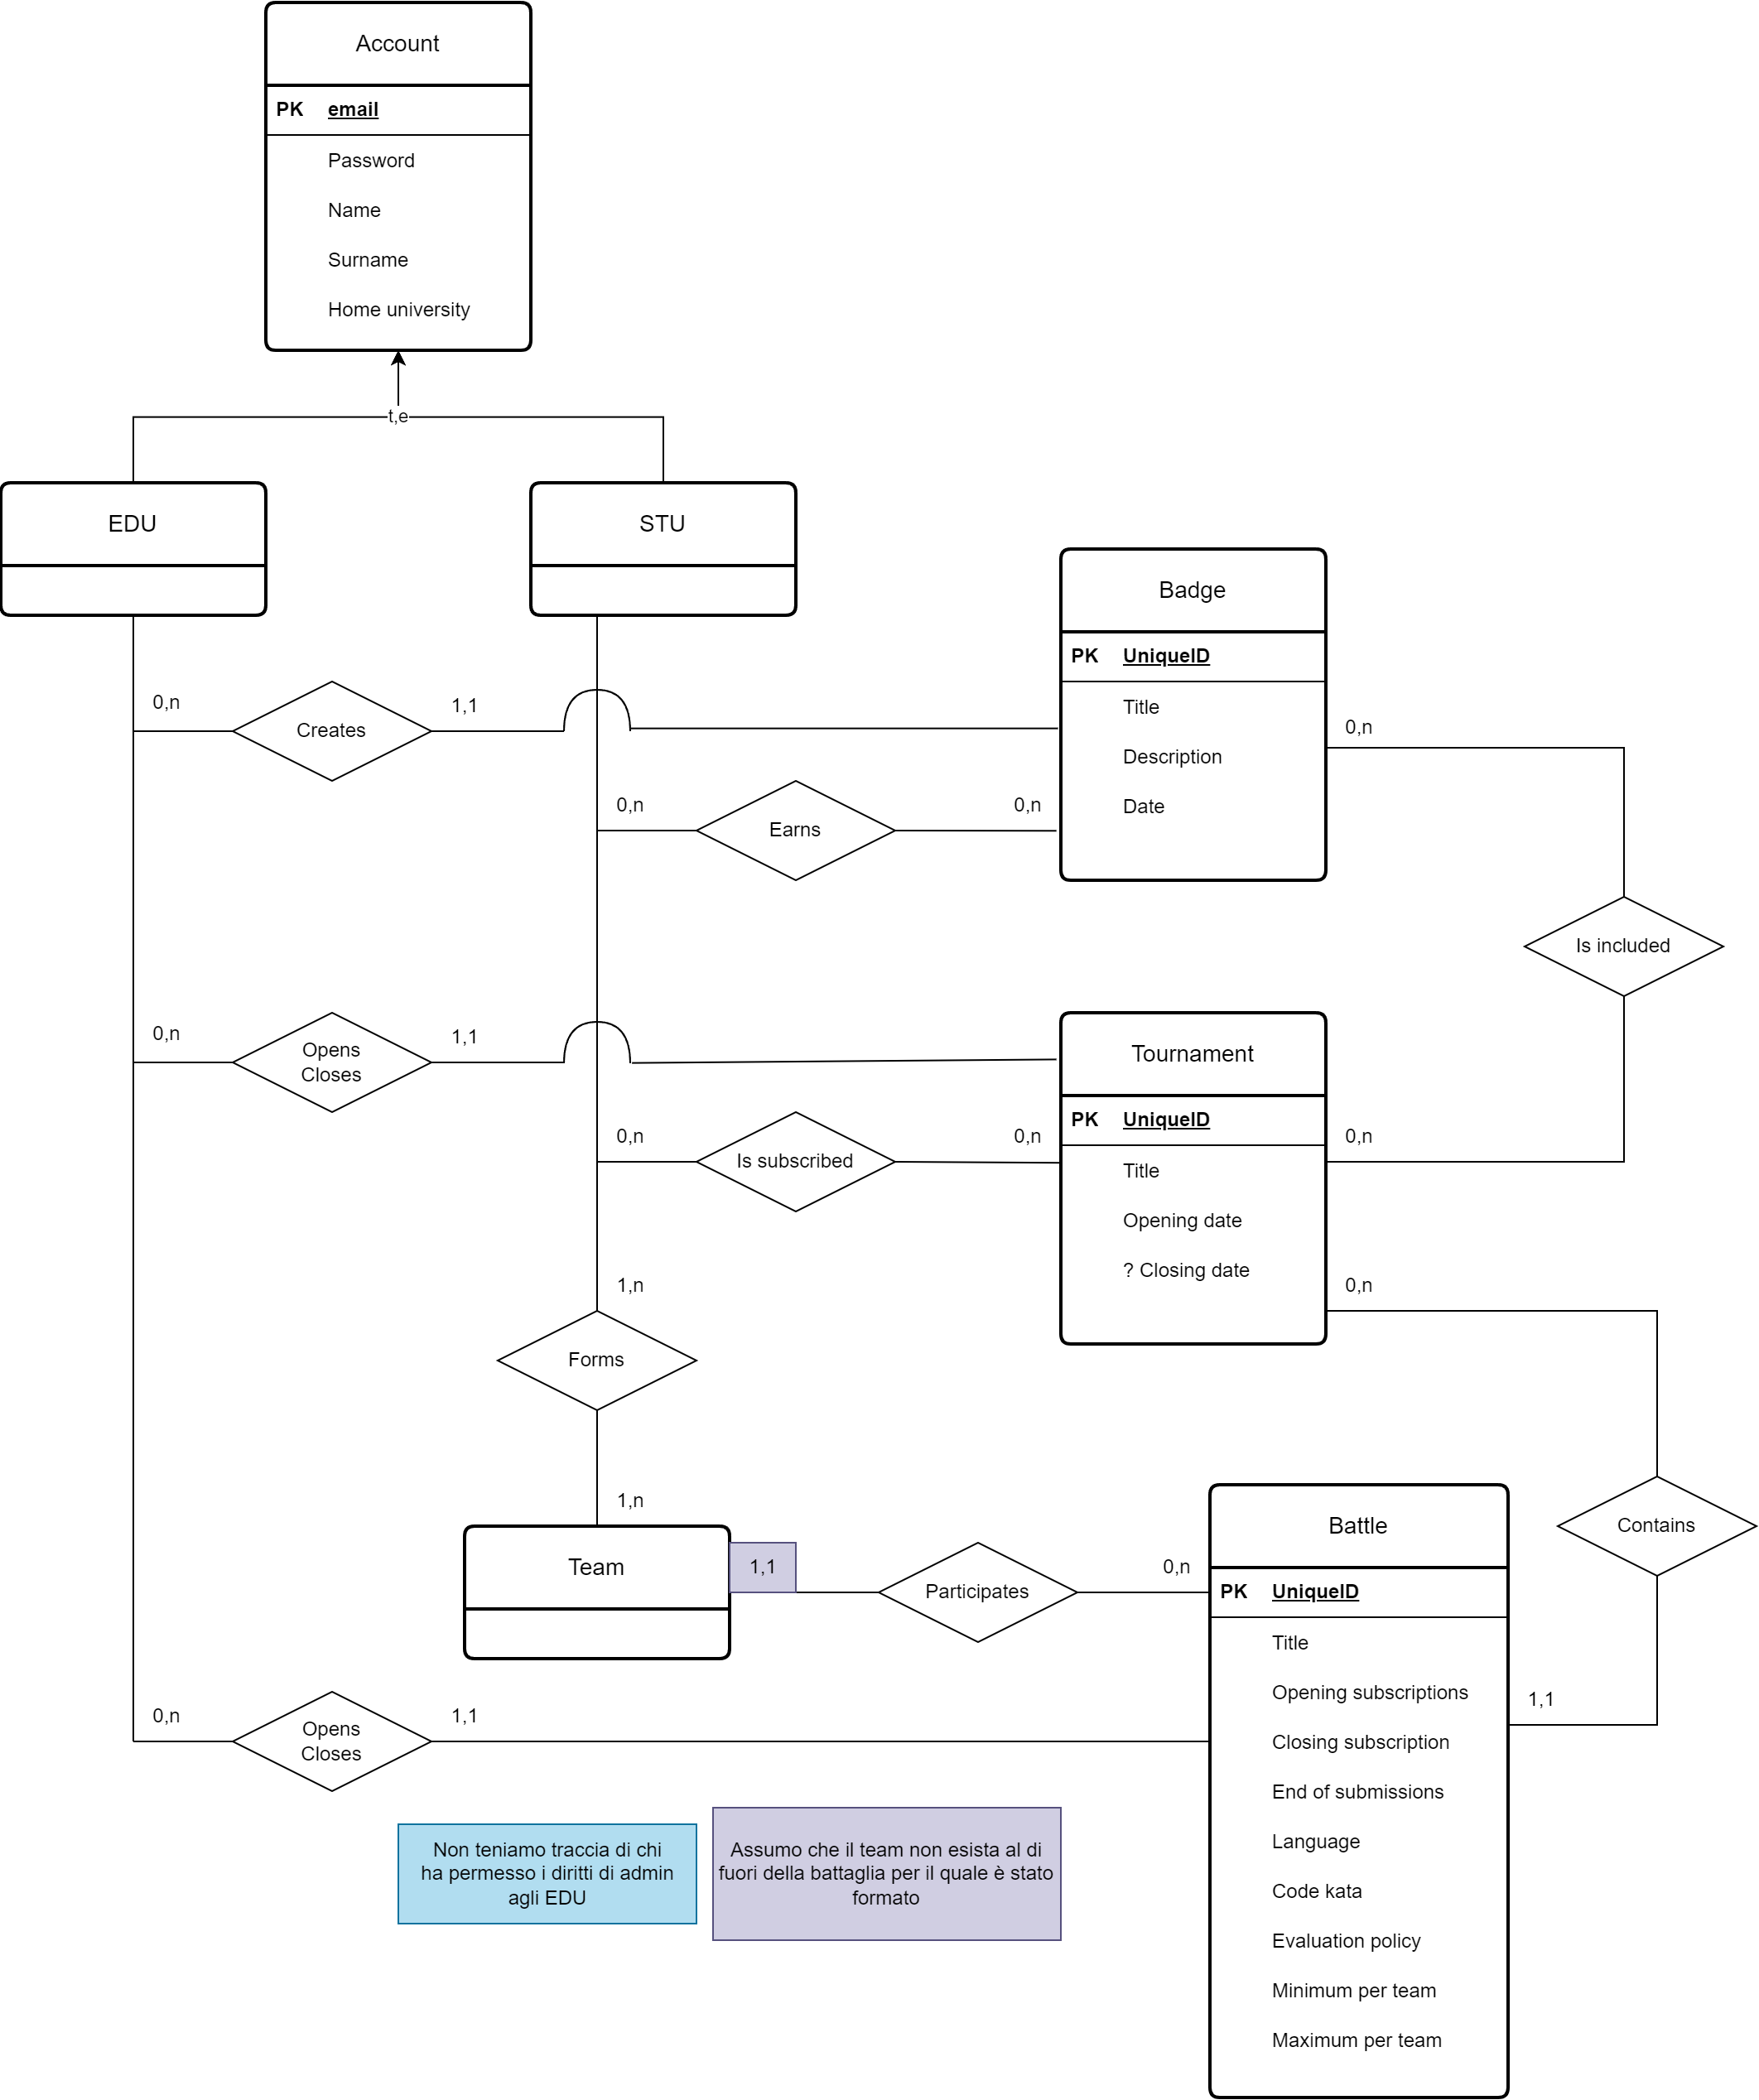
\includegraphics[width=0.75\textwidth]{images/diagrams/er_diagram.png}
    \caption{Entity-relationship diagram}
    \label{fig:er_diagram}
\end{figure}

\section{Deployment view}
The diagram \ref{fig:deployment_diagram} shows the deployment view of the system.\\\\
Our system comprises two essential components: a static web server and an application server. The static web server serves as the entry point for clients to access the SPA, while the application server furnishes the necessary APIs for the SPA's functionality. To optimize performance, we have opted for distinct solutions for these components.\\
The static web server will be hosted on a CDN (Content Delivery Network) on cloud, exploiting its edge location caches and reverse proxies to ensure rapid response times. On the other hand, the application server, containing both a business logic layer and a data tier, will find its home on a cloud provider. This decision offers numerous advantages over traditional in-house hosting, including:
\begin{itemize}
    \item \textbf{Scalability and Flexibility}: The cloud infrastructure allows for the dynamic addition or removal of resources like virtual machines, performance cores, or memory as per the evolving needs. Load balancing services further enable the application server to adapt seamlessly to changes in traffic or workload.
    \item \textbf{Security}: Enhanced security features, such as live monitoring and firewalls, contribute to safeguarding the application server against potential data breaches, cyberattacks, and other security threats.
    \item \textbf{Cost-efficiency}: The cloud provider's pay-as-you-go model ensures cost efficiency by charging only for the utilized resources. This approach helps in reducing overall costs, making it a financially prudent choice.
\end{itemize}
These attributes position a cloud provider as an ideal hosting solution for large, high-traffic applications. The selected cloud provider must respect all these features to effectively meet our system requirements.\\

\begin{figure}[ht]
    \centering
    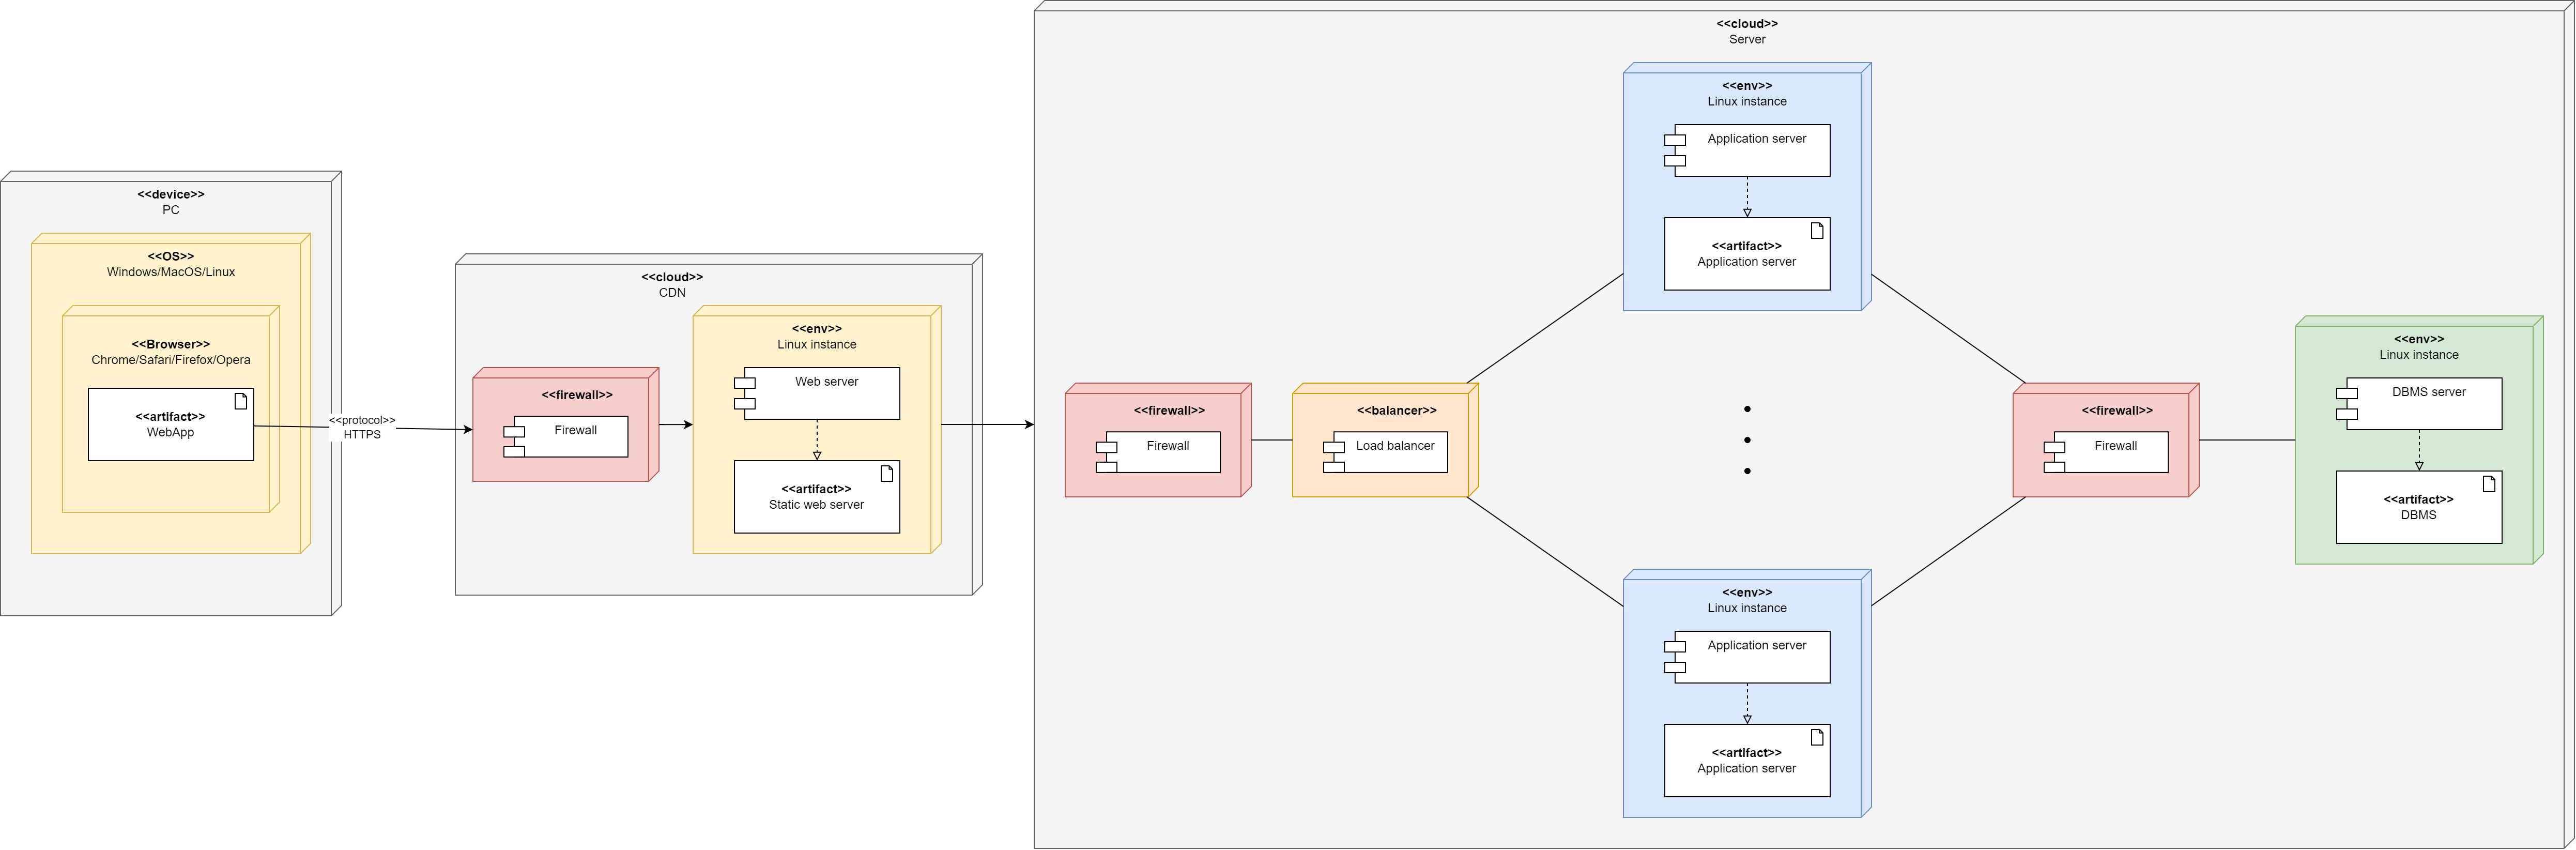
\includegraphics[width=\textwidth]{images/diagrams/deployment_view.png}
    \caption{Deployment diagram}
    \label{fig:deployment_diagram}
\end{figure}

{\color{red} mettere la cdn in mezzo, come sulle slides di tiw}

The components of the system are explaineed in the following:
\begin{itemize}
    \item \textbf{PC}: Personal computer of the user, it suffices to have a wordking O.S. and a browser installed that supports JavaScript and HTML5 in order to use the system.
    \item \textbf{CDN}: As said before, the CDN is used to host the static web server, that serves as the entry point for clients to access the SPA. It will allow it to be downloaded without affecting the performance of the main application server. The SPA is static and all of its code is run on the client's machine, so there is no need for any logic to be implemented on the CDN side.
    \item \textbf{Cloud provider}: The cloud provider is used to host the application server. It will allow the system to be scalable and flexible, to be secure and to be cost-efficient.\\
          It is composed by:
          \begin{itemize}
              \item \textbf{Load balancer}: The load balancer is used to distribute the traffic between the different instances of the application server. It is used to make the system scalable and flexible.
              \item \textbf{Application servers}: The application servers are used to host the application server. They will be in an array of instances, so that the load balancer can distribute the traffic between them. The number of instances can be changed dynamically, so that the system can adapt to the traffic. They are used to make the system scalable and flexible.
              \item \textbf{DBMS server}: The DBMS server is used to host the database.
              \item \textbf{Firewalls}: They are used to make the system secure, and are placed between the load balancer and the external world and between the application servers and the DBMS server. They provide an additional layer of security by blocking or allowing traffic based on predetermined rules. This helps to protect the system from unauthorized access or malicious attacks
          \end{itemize}
\end{itemize}


{\color{red} Da qui in avanti in questo capitolo dobbiamo prima parlarne un secondo su cosa metter (secondo me la sezione \textit{API endpoints}, visto che c'è prevalentemente server-side, dovrebbe scriverlo chi si occuperà del backend )}
\section{Runtime View}
This section describes the most important components interactions of the system.

\subsection{User login}
At the beginning the end user must log in to use the main functions of the application. The login is done by enetring the email and password. If the credentials are present in the database and correct the process will be successful and it will be able to open its dashboard, otherwise it will have to repeat the procedure. (Figure \ref{fig:RuntimeView_UserLogin})
\begin{figure}[H]
    \centering
    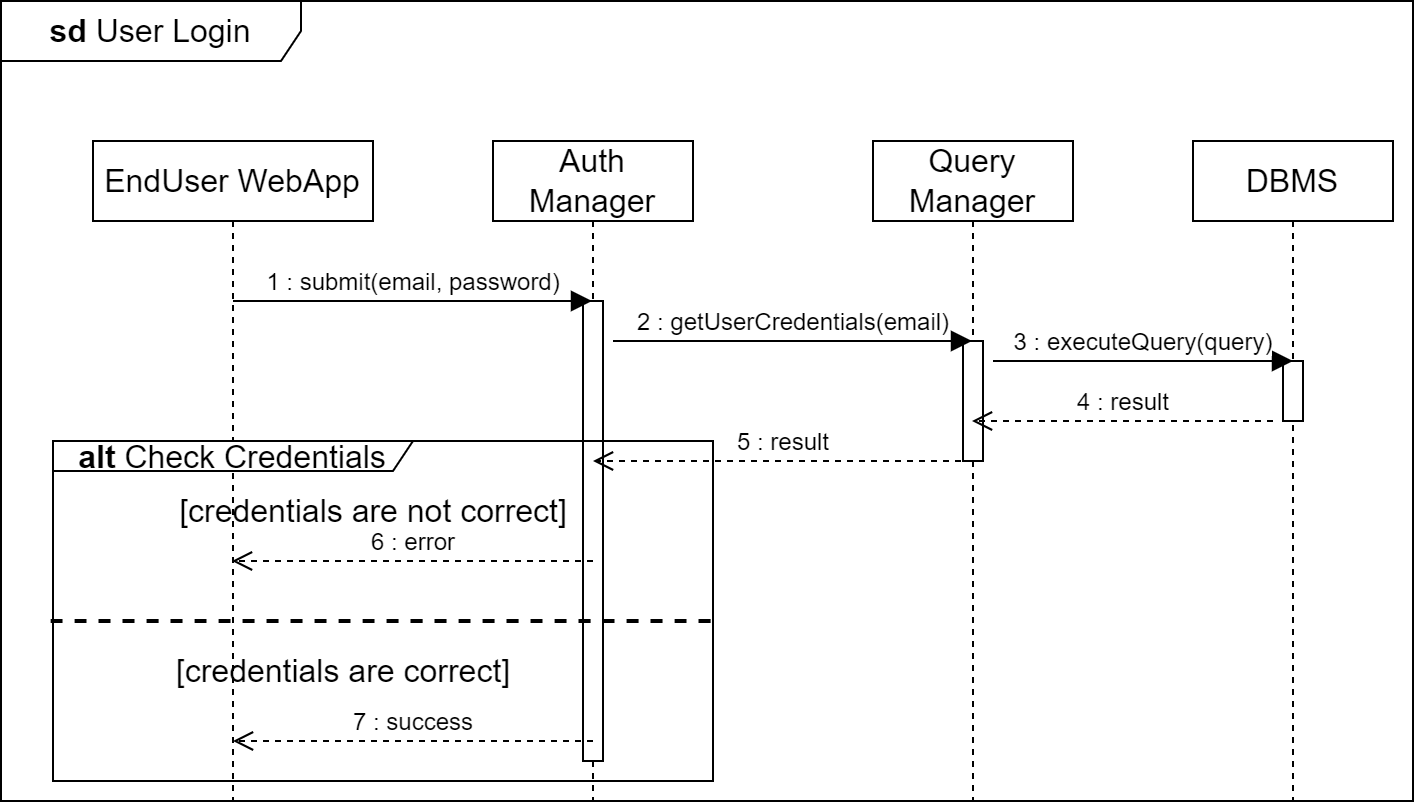
\includegraphics[width=\textwidth]{images/runtimeviews/RuntimeView_UserLogin.png}
    \caption{Runtime View of User Login Event}
    \label{fig:RuntimeView_UserLogin}
\end{figure}

\subsection{Create a tournament}
The following sequence diagram is used to explain how to create a tournament. The end user from its device can create a tournament entering the correlated details through the related component, which are sent to the database. If the tournament has been created successfully, the correlated page is created.(Figure \ref{fig:RuntimeView_CreateTournament} )
\begin{figure}[H]
    \centering
    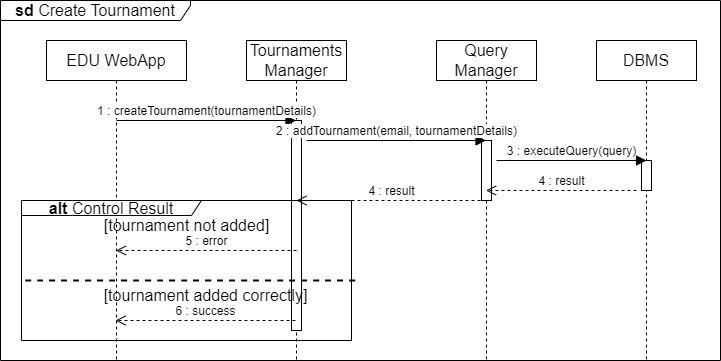
\includegraphics[width=\textwidth]{images/runtimeviews/RuntimeView_CreateTournament.png}
    \caption{Runtime View of Create a Tournament Event}
    \label{fig:RuntimeView_CreateTournament}
\end{figure}

\subsection{Create a battle}
The following sequence diagram is used to explain how to create a battle within a tournament. The end user from its device can create a battle entering the correlated details through the related component. If the user is a granted educator for the current tournament, then the details of the new battle are sent to the database and if the battle has been created successfully, the correlated page is created and all the users subscribed to the correlated tournament are notified. (Figure \ref{fig:RuntimeView_CreateBattle})
\begin{figure}[H]
    \centering
    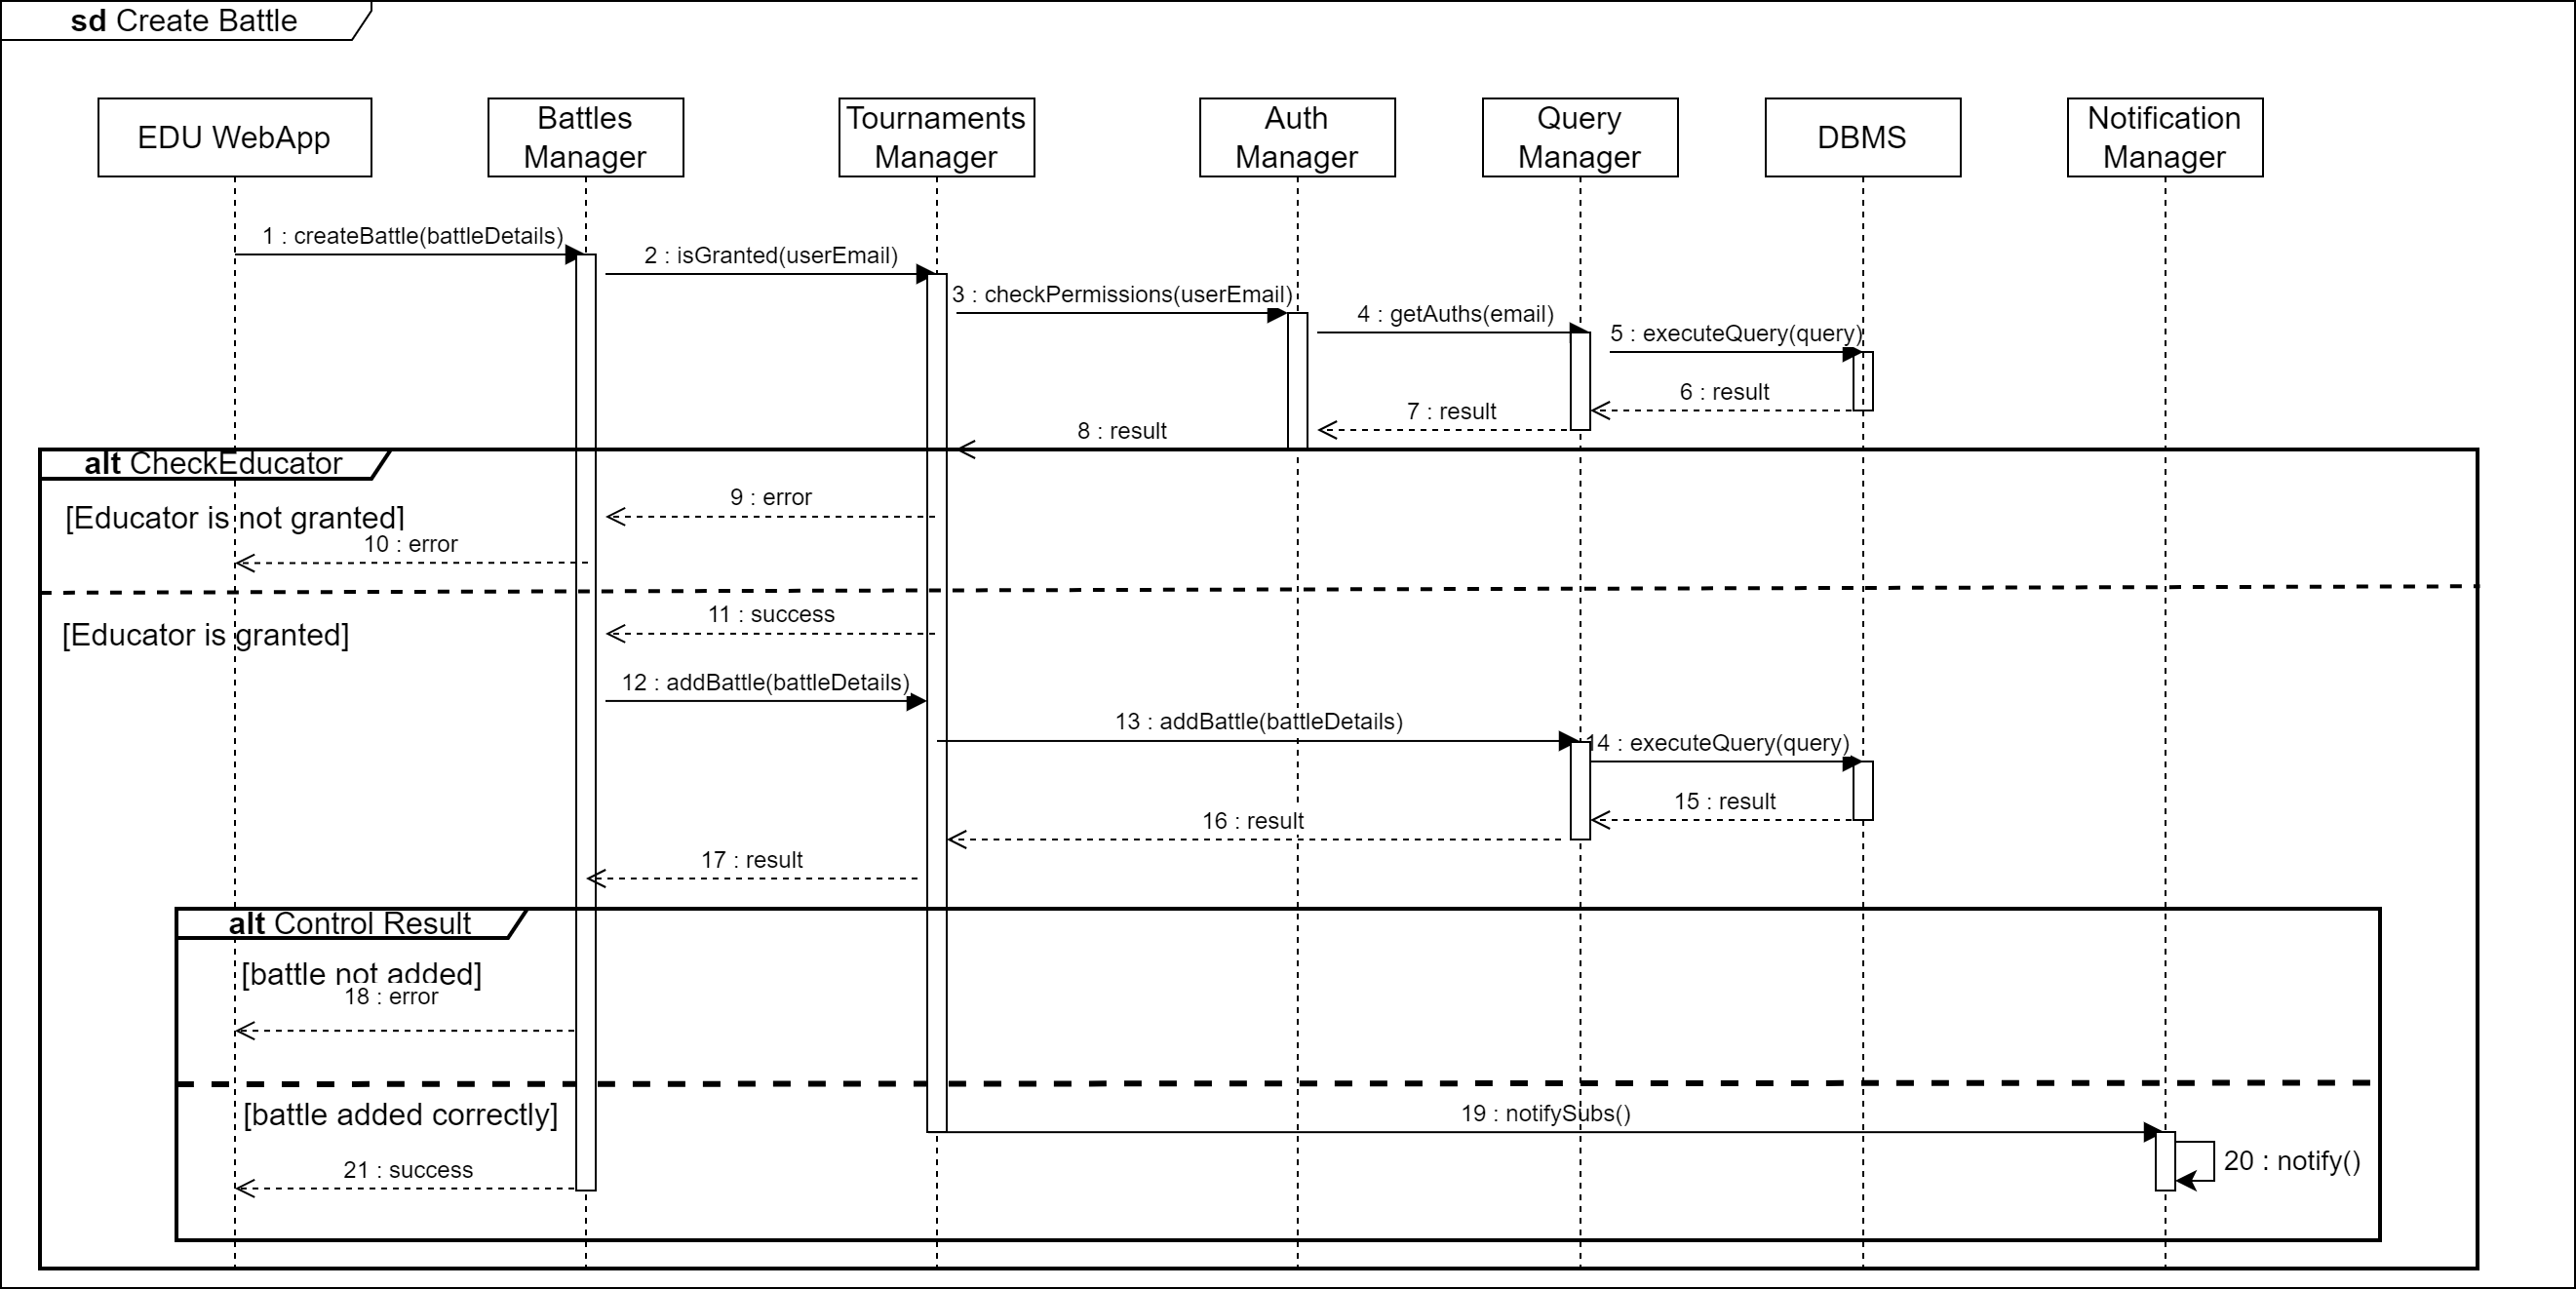
\includegraphics[width=\textwidth]{images/runtimeviews/RuntimeView_CreateBattle.png}
    \caption{Runtime View of Create a Battle Event}
    \label{fig:RuntimeView_CreateBattle}
\end{figure}

\subsection{Join a Battle Solo}
In this sequence diagram is shown how an user can subscribe to a battle. By joining the battle, the system add to the database the email of the user into the subscribed email of that battle. If the user decides to invite other members, the inserted emails are notified. (Figure \ref{fig:RuntimeView_JoinBattleSolo})
\begin{figure}[H]
    \centering
    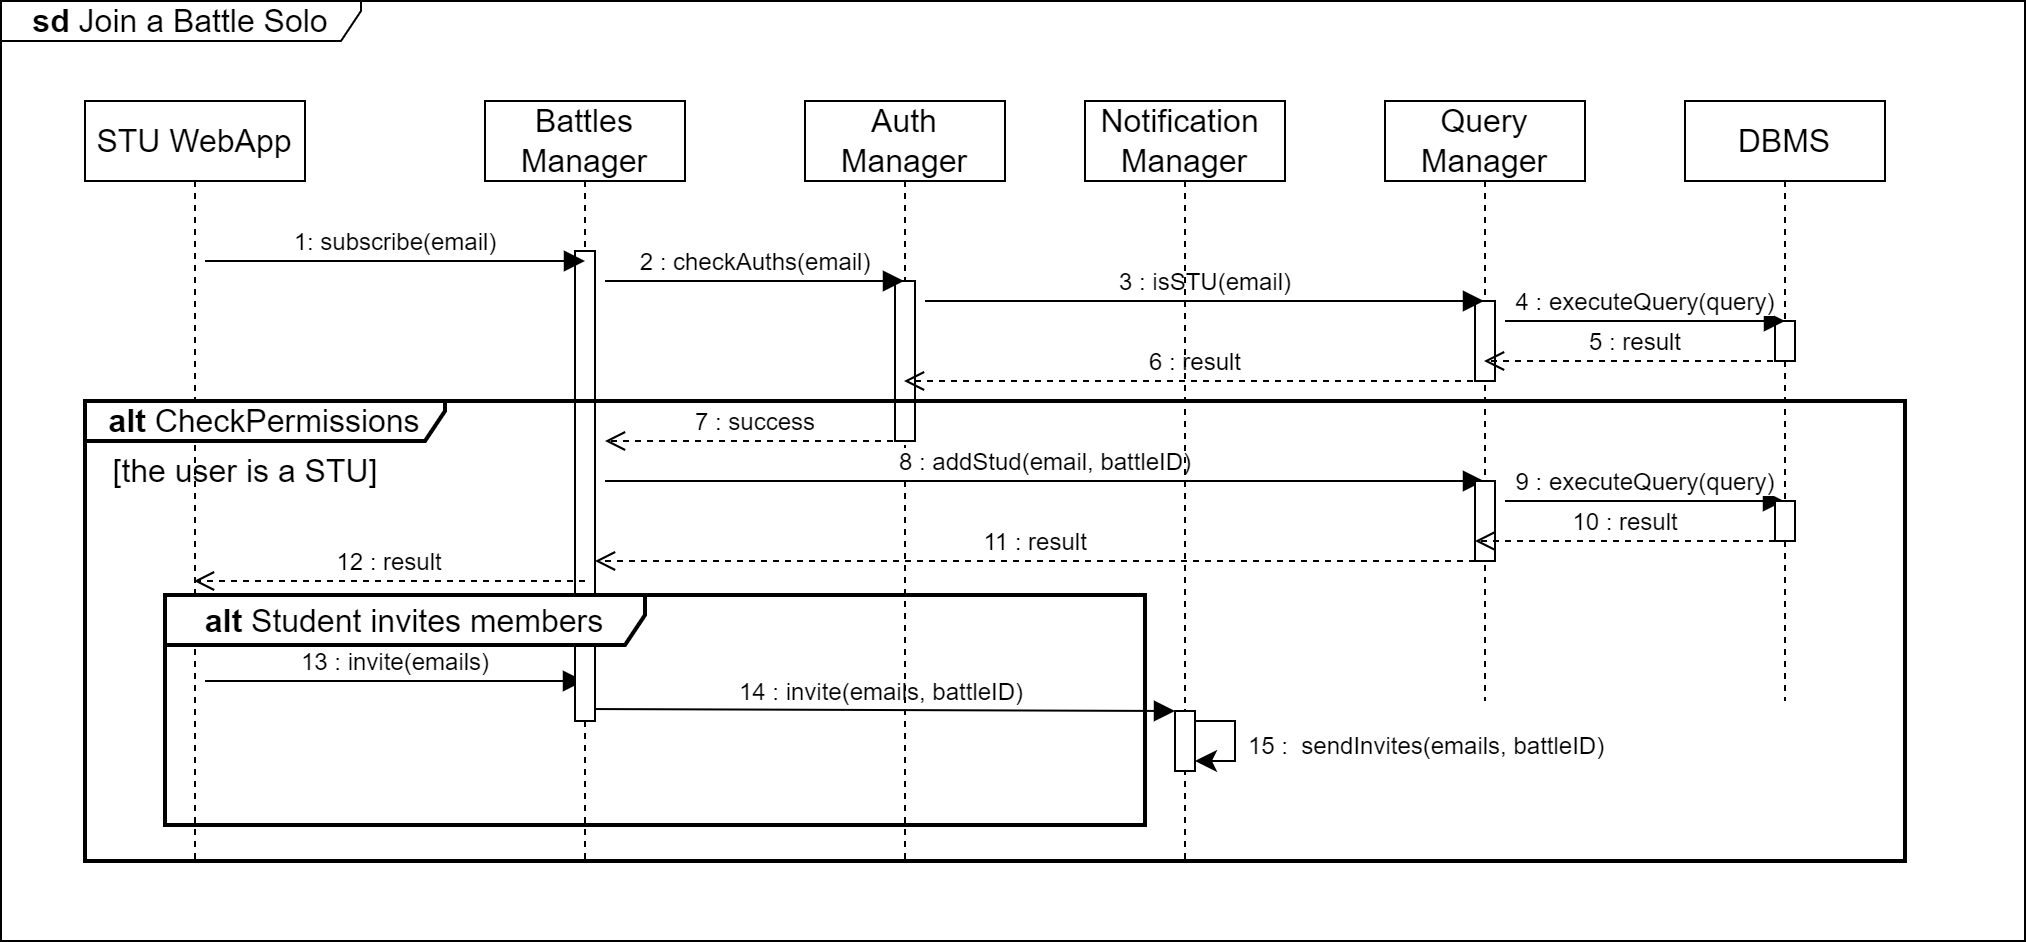
\includegraphics[width=\textwidth]{images/runtimeviews/RuntimeView_JoinBattleSolo.png}
    \caption{Runtime View of joining a Battle Solo}
    \label{fig:RuntimeView_JoinBattleSolo}
\end{figure}

\subsection{Upload code}
In this case, the GitHub API notify the system which through the related component computes the new score and update it by sending the new score to the database. Finally, the system updates the battle ranking with the new score. (Figure \ref{fig:RuntimeView_CodeUploaded})
\begin{figure}[H]
    \centering
    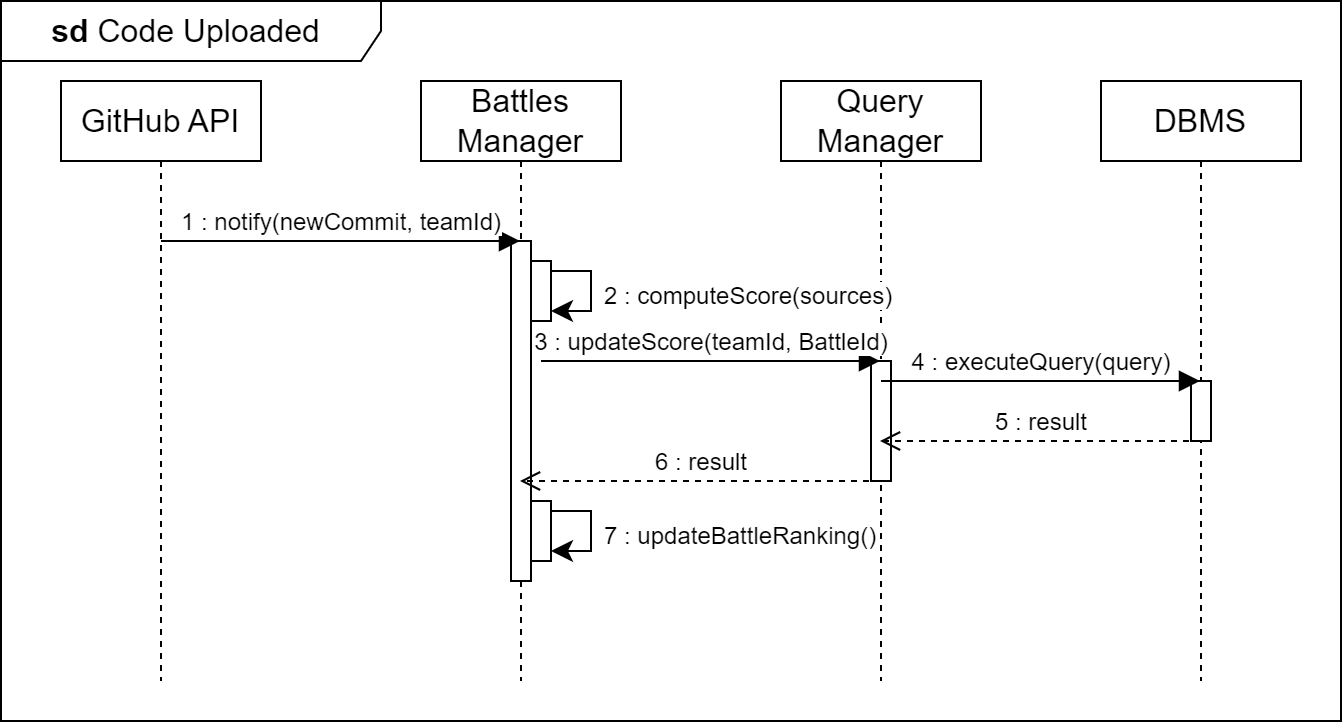
\includegraphics[width=\textwidth]{images/runtimeviews/RuntimeView_CodeUploaded.png}
    \caption{Runtime View of Notification of a new commit of a team}
    \label{fig:RuntimeView_CodeUploaded}
\end{figure}

\section{API endpoints}
% Define JavaScript language style
\lstdefinelanguage{JavaScript}{
    keywords={const, let, var, if, else, for, while, function},
    keywordstyle=\color{blue},
    commentstyle=\color{gray},
    stringstyle=\color{ForestGreen},
    morecomment=[l]{//},
    morecomment=[s]{/*}{*/},
    morestring=[b]",
    morestring=[b]'
}

% Set general listings style
\lstset{
    basicstyle=\ttfamily\footnotesize,
    showstringspaces=false,
    tabsize=2,
    breaklines=true
}

The following section describes one by one the endpoints of the APIs offered by the system.\\
For the "battle" object, the "phase" attribute is intended to be as an enumeration of 4 possible values:
\begin{itemize}
    \item 1 - Registration
    \item 2 - Code Submission
    \item 3 - Manual evaluation
    \item 4 - Finished, closed
\end{itemize}

{\color{red} Qui vi lascio tutte le api con le relative informazioni che mi sevono, poi i path per raggiungerle gestiteveli voi come vi è più comodo e fatemi sapere}

\section*{GET endpoints - General User}

\subsection*{Search for a student}
This endpoint allows the anyone who writes in the searchbox to search for a STU by name, surname or email.\\
\textbf{Method} : GET \\
\textbf{EndPoint} : api/search/student/:query \\
\textbf{URL Parameters} :
\begin{itemize}
    \item {\ttfamily{query}} : the string that the user has written in the searchbox\\
\end{itemize}
\textbf{Response} :
\begin{itemize}
    \item {\ttfamily{200}} : JSON object
          \begin{lstlisting}[language=JavaScript, label={lst:jscode}, basicstyle=\ttfamily]
[
    {
        "id": Number,
        "name": String,
        "surname": String,
    },
    ...
]
            \end{lstlisting}
    \item {\ttfamily{400}} : error String("The searchbox is empty, at least 1 character is required")
    \item {\ttfamily{401}} : error String("Unauthorized")
\end{itemize}

\subsection*{Inspect a STU's profile}
This endpoint allows the anyone who clicks on a STU's name in the search results to inspect its profile.\\ % or click on a STU's name in any point of the system
\textbf{Method} : GET \\
\textbf{EndPoint} : api/search/student/id/profile \\
\textbf{URL Parameters} :
    \begin{itemize}
        \item {\ttfamily{id}} : the id of the student the user is looking for
    \end{itemize}
\textbf{Response} : 
    \begin{itemize}
        \item {\ttfamily{200}} : JSON object
        \begin{lstlisting}[language=JavaScript, label={lst:jscode}, basicstyle=\ttfamily]
{
    "name": String,
    "surname": String,  
    "tournaments": [
        {
            "id": Number,
            "name": String
        },
        ...
    ],
    "badges": [
        {
            "id": Number,
            "name": String,
            "rank": Number[1 - 7],
            "obtained": [
                {
                    "date": String(Date),
                    "tournament": String,
                    "tournament_id": Number,
                    "battle": String,
                    "battle_id": Number
                },
                ...
            ]
        },
        ...
    ]
}
        \end{lstlisting}
        \item {\ttfamily{401}} : error String("unauthorized")
    \end{itemize}



\section*{GET endpoints - EDU}

\subsection*{Get all tournaments}
This endpoint allows the EDU to get the list of all the tournaments on the CKB platform, it will be accessed whenever the EDU clicks on the "Show all tournaments" button on the dashboard.\\
\textbf{Method} : GET \\
\textbf{EndPoint} : api/search/tournaments \\
\textbf{URL Parameters}: None \\
\textbf{Response}:
\begin{itemize}
    \item {\ttfamily{200}} : JSON object
          \begin{lstlisting}[language=JavaScript, label={lst:jscode}, basicstyle=\ttfamily]
[
    {
        "id": Number,
        //name of the tournament
        "name": String,
        // first name of the tournament creator
        "first_name": String, 
        // last name of the tournament creator
        "last_name": String,
        // if the tournament is open (true) or closed (false)
        "active": Boolean,
    },
    ...
]
        \end{lstlisting}
    \item {\ttfamily{401}}: error String("unauthorized)
\end{itemize}

\subsection*{Get owned tournaments}
This endpoint allows the EDU to get the list of the tournaments that it owns, it will be accessed every time the EDU opens the dashboard.\\

\textbf{Method} : GET \\
\textbf{EndPoint} : api/search/tournaments/:parameters \\
\textbf{URL Parameters}:
\begin{itemize}
    \item {\ttfamily{id}}: the id of the EDU that is requesting the list of the tournaments
\end{itemize}
\textbf{Response}:
\begin{itemize}
    \item {\ttfamily{200}} : JSON object
          \begin{lstlisting}[language=JavaScript, label={lst:jscode}, basicstyle=\ttfamily]
[
    {
        "id": Number,
        //name of the tournament
        "name": String,
        // first name of the tournament creator
        "first_name": String, 
        // last name of the tournament creator
        "last_name": String,
        // if the tournament is open (true) or closed (false)
        "active": Boolean,
    },
    ...
]
            \end{lstlisting}
    \item {\ttfamily{401}} : error String("Unauthorized")
\end{itemize}

\subsection*{Get tournament details}
This endpoint allows the EDU to get the details of a tournament, it will be accessed when an EDU selects a tournament from the list of the tournaments in the dashboard.\\
\textbf{Method} : GET \\
\textbf{EndPoint} : api/search/tournaments/:parameters \\
\textbf{URL Parameters}:
\begin{itemize}
    \item {\ttfamily{id}} : id of the tournament
    \item {\ttfamily{edu\_id}}: the id of the EDU that is requesting the details of the tournament
\end{itemize}
\textbf{Response}:
\begin{itemize}
    \item {\ttfamily{200}} : JSON object
          \begin{lstlisting}[language=JavaScript, label={lst:jscode}, basicstyle=\ttfamily]
[
    {
        "id": Number,
        "name": String,
        "active": Boolean,
        "admin": Boolean,
        "battles": [
            {
                "id": Number,
                "name": String,
                "language": String,
                "participants": Number,
                "phase": Number[1 - 4],
                // Time remaining in the current phase
                "remaining": String(Date)
            },
            ...
        ],
        "ranking": [
            {
                "id": Number,
                "name": String,
                "points": Number
            },
            ...
        ],
    }
]
            \end{lstlisting}
    \item {\ttfamily{401}} : error String("Unauthorized")
\end{itemize}

\subsection*{Get battle details}
This endpoint allows the EDU to get the details of a battle, it will be accessed when an EDU selects a battle from the list of the battles in a tournament view.\\

\textbf{Method} : GET \\
\textbf{EndPoint} : api/search/tournament/:id/battles/:parameters \\
\textbf{URL Parameters}:
\begin{itemize}
    \item {\ttfamily{id}}: the id of the battle that the EDU wants to get the details of
    \item {\ttfamily{edu\_id}}: the id of the EDU that is requesting the details of the battle
\end{itemize}
\textbf{Response}:
\begin{itemize}
    \item {\ttfamily{200}} : JSON object
          \begin{lstlisting}[language=JavaScript, label={lst:jscode}, basicstyle=\ttfamily]
[
    {
        "id": Number,
        "title": String,
        "description": String,
        "language": String,
        "opening": String(Date),
        "registration": String(Date),
        "closing": String(Date),
        "min_group_size": Number,
        "max_group_size": Number,
        "link": String,
        "phase": Number[1 - 4],
        "tournament_name": String,
        "tournament_id": Number,
        "admin": Boolean,
        // Could be reduntant with phase, but it's easier to check
        "manual": Boolean,
        "ranking": [
            {
                "id": Number,
                "name": String,
                "score": Number
            },
            ...
        ],
    }
]
            \end{lstlisting}
    \item {\ttfamily{401}} : error String("Unauthorized")
\end{itemize}

\subsection*{Get the list of groups for the manual evalation}
This endpoint allows the EDU to get the list of the groups subscribed to a battle in the "manual evaluation" stage, and for each group that has already been evaluated it provides the score that it has obtained.\\
\textbf{Method} : GET \\
\textbf{EndPoint} : api/search/tournament/:tournament\_id/battles/:battle\_id/:manualEvaluation=true\&phase=3 \\
\textbf{URL Parameters}:
\begin{itemize}
    \item {\ttfamily{tournament\_id}} : the id of the tournament of the correlated battle
    \item {\ttfamily{battle\_id}} : the id of the battle that the EDU wants to get the list of the codes to evaluate of
    \item {\ttfamily{manualEvaluation}} : it is a parameter that represent the boolean variable "manual" of the battle
    \item {\ttfamily{phase}} : it is a parameter that represents the phase in which a specific battle is. In this case, the battle must be in phase 3, which corresponds to the manual evalation
\end{itemize}
\textbf{Response}:
\begin{itemize}
    \item {\ttfamily{200}} : JSON object
          \begin{lstlisting}[language=JavaScript, label={lst:jscode}, basicstyle=\ttfamily]
[
    {
        "id": Number,
        "team": String,
        "score"?: Number
    },
    ...
]
        \end{lstlisting}
    \item {\ttfamily{401}} : String("unauthorized")
\end{itemize}

\subsection*{Evaluate code}
code.js\\
This endpoint allows the EDU to evaluate a code, it will be accessed when an EDU clicks on the "Evaluate" button from the table of the codes to evaluate.\\

\textbf{Method} : GET \\
\textbf{EndPoint} : api/search/tournament/:tournament\_id/battles/:battle\_id/:team\_id     \\
\textbf{URL Parameters}:
\begin{itemize}
    \item {\ttfamily{tournament\_id}} : the id of the tournament of the correlated battle
    \item {\ttfamily{team\_id}}: the id of the group that the EDU wants to evaluate
    \item {\ttfamily{battle\_id}}: the id of the battle that the EDU wants to evaluate
\end{itemize}
\textbf{Response}:
\begin{itemize}
    \item {\ttfamily{200}} : JSON object
          \begin{lstlisting}[language=JavaScript, label={lst:jscode}, basicstyle=\ttfamily]
{
    "group_id": Number,
    "battle_id": Number,
    "language": String,
    // Name of the group
    "name": String,
    // Score of the group, null if not evaluated yet
    "score"?: Number,
    // Code of the group. The url links to the file
    "code": String(url)
}
    \end{lstlisting}
    \item {\ttfamily{401}} : error String("unauthorized")
\end{itemize}



\section*{GET endpoints - STU}

\subsection*{Get subscribed tournaments}
This endpoint allows the STU to get the list of the tournaments that it is subscribed to, it will be accessed every time the STU opens the dashboard.\\

\textbf{Method} : GET \\
\textbf{EndPoint} : api/search/tournament/:subscribed=email     \\
\textbf{URL Parameters}:
    \begin{itemize}
        \item {\ttfamily{email}} : the email of the user actually logged into the platform
    \end{itemize}

\textbf{Response}:
    \begin{itemize}
        \item {\ttfamily{200}} : JSON object 
        \begin{lstlisting}[language=JavaScript, label={lst:jscode}, basicstyle=\ttfamily]
[
    {
        "id": Number,
        "name": String,
        // first name of the tournament creator
        "first_name": String,
        // last name of the tournament creator
        "last_name": String,
        // if the tournament is open (true) or closed (false)
        "active": Boolean,
    },
    ...
]
            \end{lstlisting}
        \item {\ttfamily{401}} : error String("unauthorized") 
    \end{itemize}
\subsection*{Get unsubscribed tournaments}
This endpoint allows the STU to get the list of the tournaments that it is not subscribed to, it will be accessed every time the STU opens the dashboard.\\
\textbf{Method} : GET \\
\textbf{EndPoint} : api/search/tournament/:subscribed!=email     \\
\textbf{URL Parameters}:
    \begin{itemize}
        \item {\ttfamily{email}} : the email of the user actually logged into the platform
    \end{itemize}

\textbf{Response}:
    \begin{itemize}
        \item {\ttfamily{200}} : JSON object
        \begin{lstlisting}[language=JavaScript, label={lst:jscode}, basicstyle=\ttfamily]
[
    {
        "id": Number,
        "name": String,
        "daysLeft": Number,
    },
    ...
]
        \end{lstlisting}
        \item {\ttfamily{401}} : error String("unauthorized") 
        \end{itemize}

\subsection*{Get tournament details}
This endpoint allows the STU to get the details of a tournament, it will be accessed when a STU selects a tournament from the list of the tournaments in the dashboard.\\
\textbf{Method} : GET \\
\textbf{EndPoint} : api/search/tournament/STU=true\&id=tournament\_id\\
\textbf{URL Parameters}:
        \begin{itemize}
            \item {\ttfamily{STU}} : it is needed to retrieve the correct object for a STU
            \item {\ttfamily{tournament\_id}} : this is the id of the tournament the user is looking for
        \end{itemize}
\textbf{Response}:
        \begin{itemize}
            \item {\ttfamily{200}} : JSON object
            \begin{lstlisting}[language=JavaScript, label={lst:jscode}, basicstyle=\ttfamily]
[
    {
        "id": Number,
        "name": String,
        "active": Boolean,
        "subscribed": Boolean,
        "battles": [
            {
                "id": Number,
                "name": String,
                "language": String,
                "participants": Number,
                "subscribed": Boolean,
                "score"?: Number,
                "phase": Number[1 - 4],
                // Time remaining in the current phase
                "remaining": String(Date)
            },
            ...
        ],
        "ranking": [
            {
                "id": Number,
                "name": String,
                "points": Number
            },
            ...
        ]
    }
]
            \end{lstlisting}
            \item {\ttfamily{401}} : error String("unauthorized")
        \end{itemize}


\subsection*{Get battle details}
This endpoint allows the STU to get the details of a battle, it will be accessed when a STU selects a battle from the list of the battles in a tournament view.\\
\textbf{Method} : GET \\
\textbf{EndPoint} : api/search/tournament/STU=true\&id=battle\_id\\
\textbf{URL Parameters}:
\begin{itemize}
    \item {\ttfamily{STU}} : it is needed to retrieve the correct object for a STU
    \item {\ttfamily{battle\_id}} : this is the id of the battle the user is looking for
\end{itemize}
\textbf{Response} : 
    \begin{itemize}
        \item {\ttfamily{200}} : JSON object
        \begin{lstlisting}[language=JavaScript, label={lst:jscode}, basicstyle=\ttfamily]
[
    {
        "id": Number,
        "title": String,
        "description": String,
        "language": String,
        "opening": String(Date),
        "registration": String(Date),
        "closing": String(Date),
        "min_group_size": Number,
        "max_group_size": Number,
        "link": String,
        "phase": Number[1 - 4],
        "tournament_name": String,
        "tournament_id": Number,
        "ranking": [
            {
                "id": Number,
                "name": String,
                "score": Number
            },
            ...
        ]
    }
]
        \end{lstlisting} 
        \item {\ttfamily{401}} : error String("unauthorized")
    \end{itemize}

\section{Component interfaces}
In this diagram are displayed all the functions that each component uses to communicate with other components. In particular, the blue interfaces are external APIs in which at this level of abstraction do not require to be detailed as the other interfaces. The interfaces contains both the operations for STU users and EDU users. 
\begin{figure}[H]
    \centering
    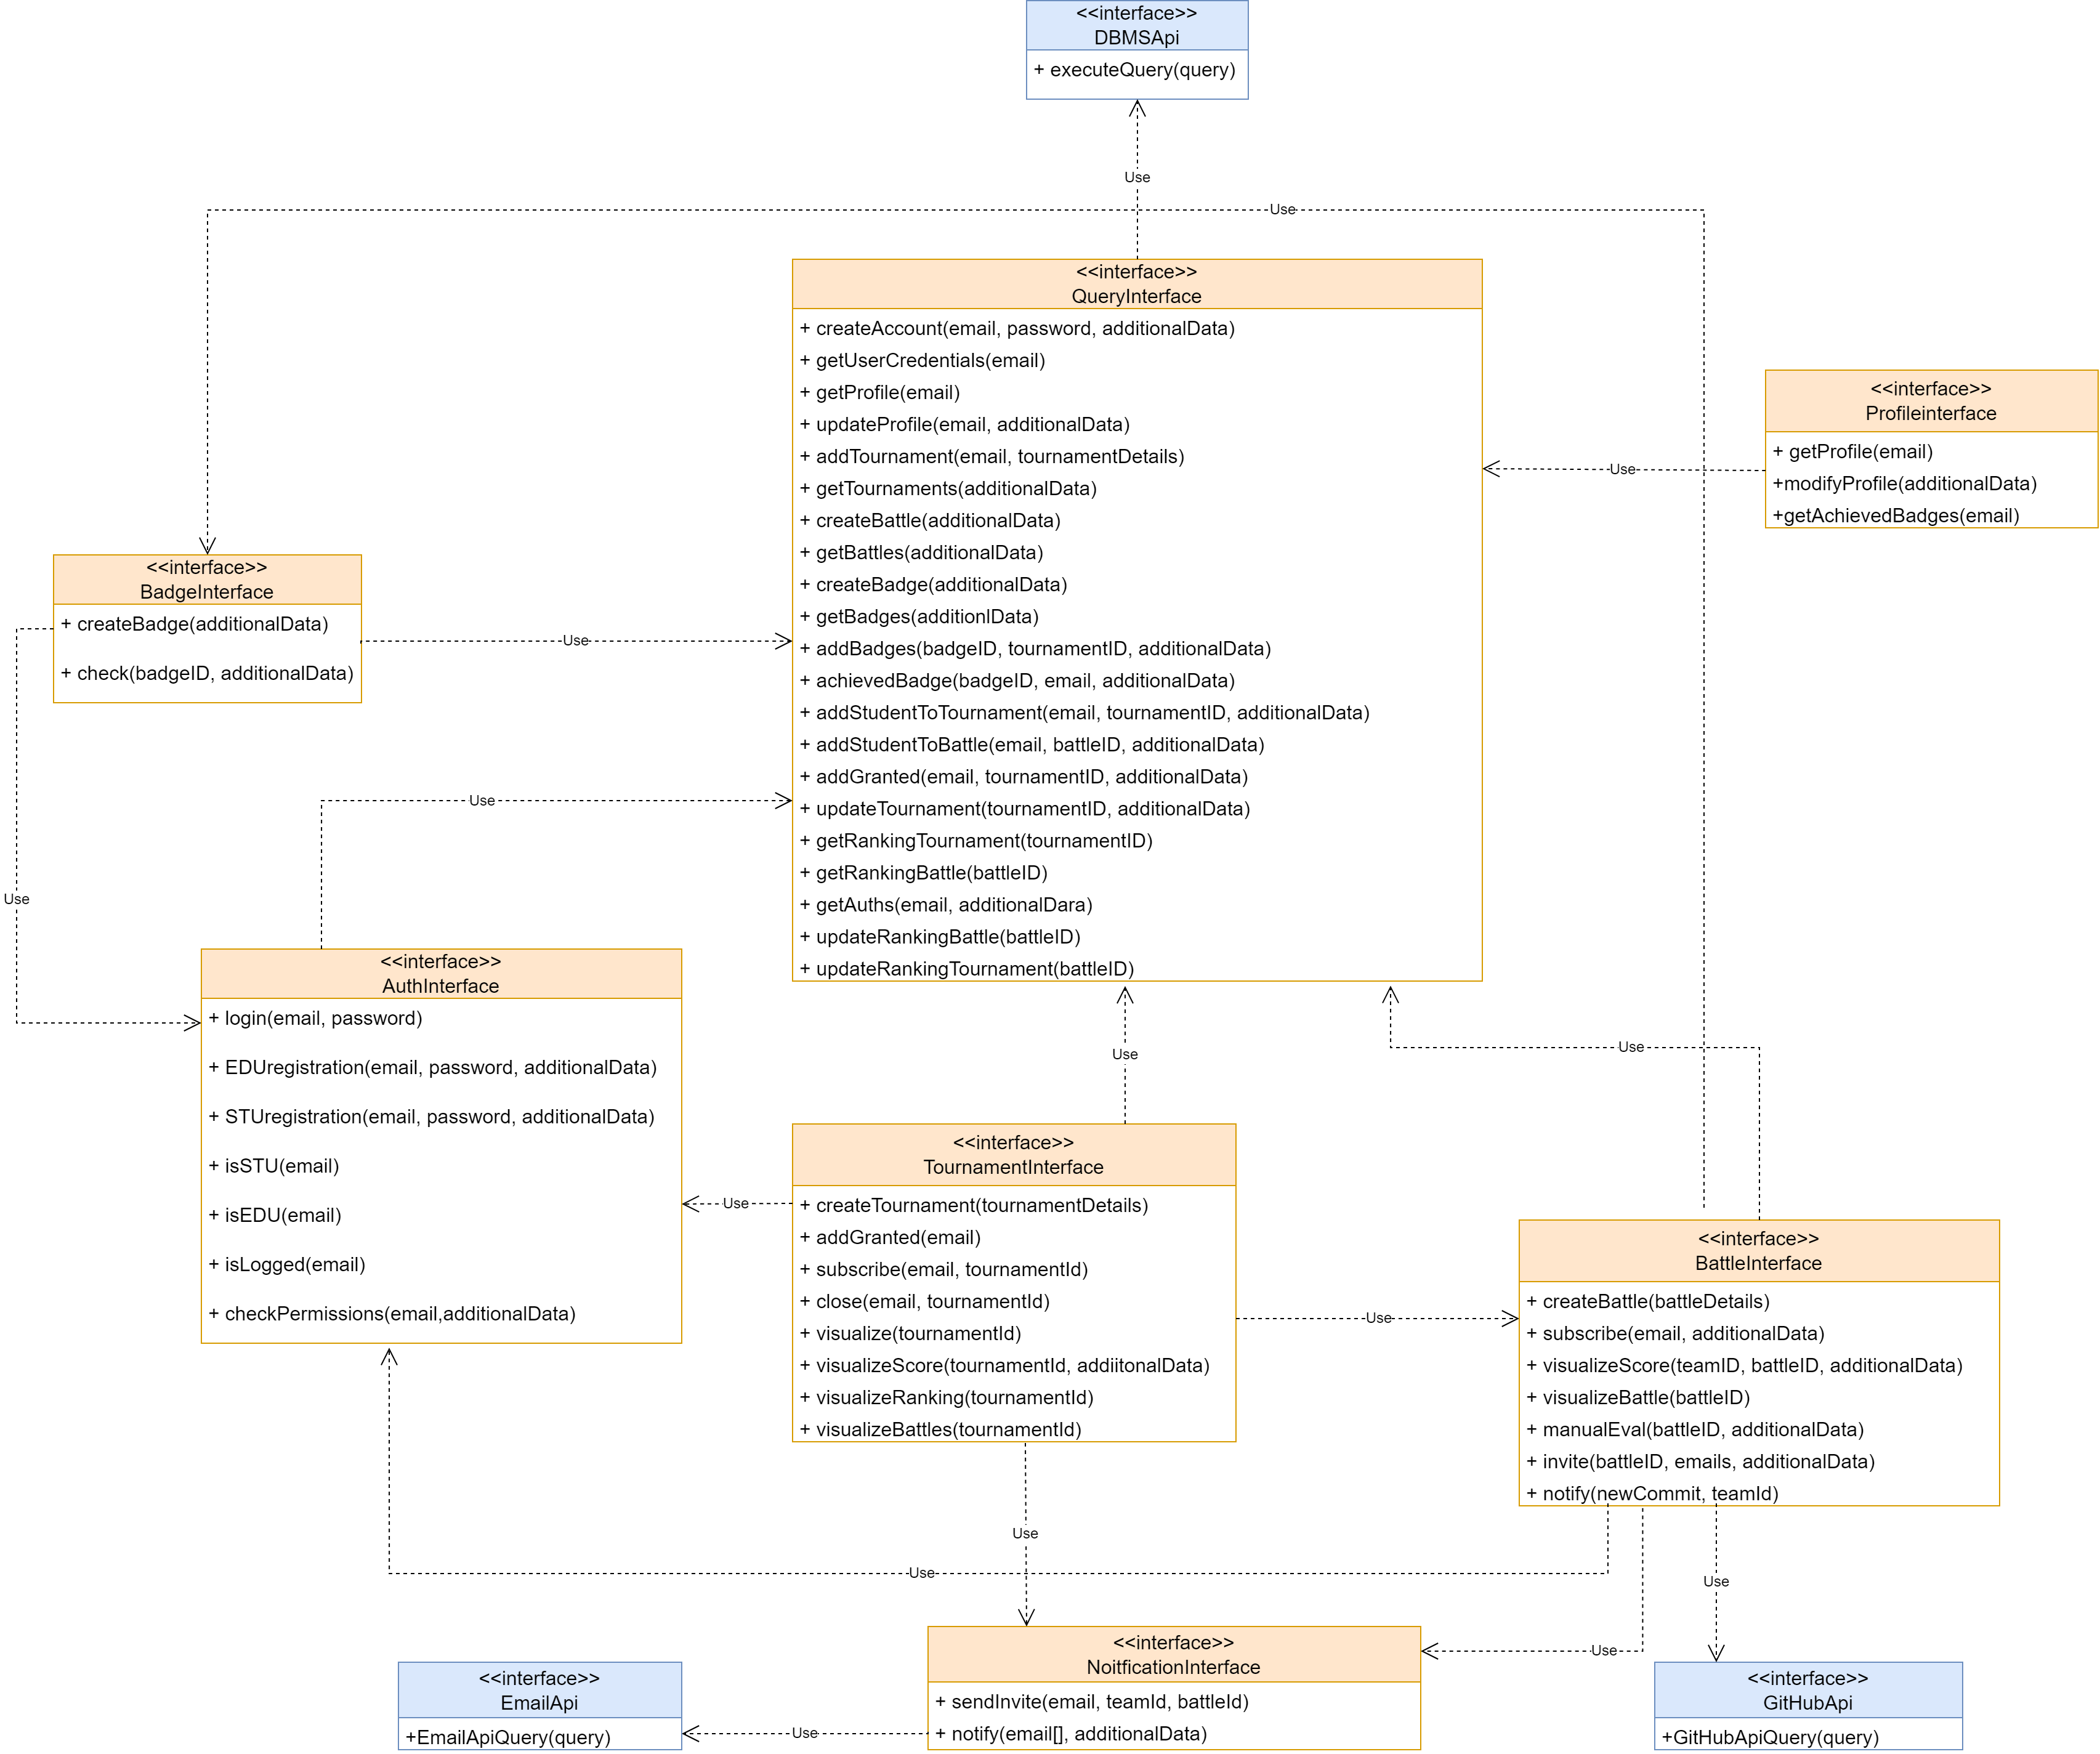
\includegraphics[width=\textwidth]{images/diagrams/ComponentInterfaces.png}
    \caption{Component interfaces diagram}
\end{figure}
\section{Other design decisions}
\subsection{Web Application}
As the platform's primary functionality is closely tied to coding activities, it is expected that users will predominantly employ personal computers, so there is no need to develop a mobile application, which would require a significant amount of additional work.\\
Instead, the system will be accessible through a web application, that is much easier to develop, maintain and being accessed by the users.

\subsection{Single Page Application}
The system will be developed as a Single Page Application (SPA), that is a web application that interacts with the user by dynamically rewriting the current web page with new data from the web server, instead of the default method of the browser loading entire new pages.\\
This approach will allow the system to be more responsive and to be more similar to a desktop application, since the user will not have to wait for the entire page to be reloaded every time he performs an action. Furthermore, it will allow the system to be more efficient, since the server will not have to send the entire page every time the user performs an action, but only the data that has changed, leaving the client to render the page.

\subsection{Relational Database}
We selected a relational database for our system design because it is effective at storing structured data, granting data integrity, and providing fast query performance. It can also be easily scaled to handle large amounts of data and support many concurrent users. The database allows us to store and retrieve information efficiently, while also ensuring that the data is accurate and consistent

\subsection{RESTful API}
We have chosen to implement a RESTful API for our system because it is a simple, lightweight, and flexible architecture that is easy to understand and use. It is also scalable and reliable, making it ideal for our application.\\

